\columnbreak

\part{Filtering Algorithms}
\setcounter{section}{0}

\section{Filters \& Convolution}

\Def[Filter] A function $F: l^\infty(\Z) \rightarrow l^\infty(\Z)$ where $l^\infty(\Z)$ is the space of bounded infinite sequences
$$
l^\infty(\Z) = \left\{\left(x_{j}\right)_{j \in \Z}: \sup \left|x_{j}\right|<\infty\right\}
$$

\Def[LT-FIR] A Filter that is: \begin{itemize}
	\item Linear
	\item Time-Invariant: Shifting the input in time leads to the same output shifted in time.
	\item Finite: $\exists M \forall j : x_j=0 \text{ if } \abs{j}>M \implies \exists N \forall j : y_j=0 \text{ if } \abs{j}>N$
	\item Causal: The output does not start before the input.
\end{itemize}
Such a filter is uniquely characterized by its \textbf{Impulse response}: $$F(\delta_{j, 0}) = \dots, 0, h_0, h_1, \dots, h_{n-1}, 0, \dots$$
For inputs $\vx \in \R^m$ we get outputs $\vy \in \R^{m+n-1}$
$$
\left[\begin{array}{l}
y_{0} \\
y_{1} \\
y_{2} \\
y_{3} \\
y_{4} \\
y_{5} \\
y_{6} \\
\end{array}\right]=\left[\begin{array}{cccc}
h_{0} & 0 & 0 & 0 \\
h_{1} & h_{0} & 0 & 0 \\
h_{2} & h_{1} & h_{0} & 0 \\
h_{3} & h_{2} & h_{1} & h_{0} \\
0 & h_{3} & h_{2} & h_{1} \\
0 & 0 & h_{3} & h_{2} \\
0 & 0 & 0 & h_{3} \\
\end{array}\right]\left[\begin{array}{l}
x_{0} \\
x_{1} \\
x_{2} \\
x_{4}
\end{array}\right]
$$

\Def[Discrete Convolution] A Filter where given $\mathbf{x}=\left[x_{0}, \ldots, x_{m-1}\right]^{\top} \in \mathbb{K}^{m}, \mathbf{h}=\left[h_{0}, \ldots, h_{n-1}\right]^{\top} \in \mathbb{K}^{n}$ their DCONV is the vector $\mathbf{y} \in \mathbb{K}^{m+n-1}$ with components.
$$y_{k}=\sum_{j=0}^{m-1} h_{k-j} x_{j}$$

\Def[Periodic Convolution] Given two $n$-periodic signals $\left(u_{k}\right)_{k \in \mathbb{Z}},\left(x_{k}\right)_{k \in \mathbb{Z}}$ PCONV yields the $n$-periodic signal:
$$\left(y_{k}\right):=\left(u_{k}\right) *_{n}\left(x_{k}\right), y_{k}:=\sum_{j=0}^{n-1} u_{k-j} x_{j}$$
PCONV can be represtend by a matrix $$\mathbf{C}=\left[c_{i j}\right]_{i, j=1}^{n}, c_{i j} = u_{j-i}$$. Such a matrix is called \textbf{circulant}. The vector $\vu$ s.t. $\MC = \operatorname{circul}(\vu)$ corresponds to $\MC_{:,1}$.

\section{Discrete Fourier Transform}
The Fourier Matrix for inputs $\vy \in \C^{n}$ is given by
$$ \MF_n = \left[\omega_{n}^{l j}\right]_{l, j=0}^{n-1} \in \mathbb{C}^{n, n} \quad \omega_{n} = \exp\left(\frac{-2\pi i}{n}\right)$$
and $\mathrm{DFT}_{n}(\mathbf{y}):=\mathbf{F}_{n} \vy = \left[\sum_{j=0}^{n-1} y_{j} \omega_{n}^{k j}\right]_{k=0}^{n-1}$. \\ Properties include
$$\MF_{n}^{-1}=\frac{1}{n} \MF_{n}^{\Hm}=\frac{1}{n} \overline{\MF}_{n}$$

\sep
\Method[Frequency Filtering]
The columns $\vv_k$ of $\MF_n$ are trigonometric basis vectors, where 
$$\vv_k = \left[\cos \left(\tcg{j\frac{2 \pi}{n}}\cdot \tcp{k}\right)+\boldsymbol{\imath} \sin \left(\frac{2 \pi j k}{n}\right)\right]_{j=0}^{n-1}$$
$\tcg{k}$ is the 'frequency' and $\tcp{j2\pi/n}$ is  the sample point.
Hence the $\mathrm{DFT}_{n}$ is a basis transformation $$B_E \leftrightarrow B_{trig}$$
Denoising and low/high filters can be implemented by manipulating the signal in the frequency domain.
Given the $n$ coeffiecient $c_j$ we can analyse the strength of frequencies by plotting $\abs{c_j}^2, 0\leq j\leq n/2$, since $\vv_k = \vv_{n-k}, k=0\dots n-1$.

\sep

\Lemma[Diagonalizing circulant matrices] \\
For any circulant matrix $\MC \in \C^{n,n}$ we have 
\begin{align*}
&\mathbf{C}=\mathbf{F}_{n}^{-1} \operatorname{diag}\left(d_{1}, \ldots, d_{n}\right) \mathbf{F}_{n}, \\ 
&\left[d_{0}, \ldots, d_{n-1}\right]^{\top}=\mathbf{F}_{n}\left[u_{0}, \ldots, u_{n-1}\right]^{\top}
\end{align*}
In other words, the columns of $\MF_n$ are eigenvectors of $\MC$. \\

\Theorem[Convolution Theorem] 
Periodic convolution in the time-domain equals to multiplication in the frequency-domain.
$$
(\mathbf{u}) *_{n}(\mathbf{x})=\mathbf{F}_{n}^{-1}\left[\left(\mathbf{F}_{n} \mathbf{u}\right)_{j}\left(\mathbf{F}_{n} \mathbf{x}\right)_{j}\right]_{j=1}^{n}
$$
Implementation Speedup: $\BigO(n^2) \rightarrow \BigO(n \log_2(n))$
\sep

\Theorem[2D DFT] Is given by 
$$
\mathbf{C}=\mathbf{F}_{m}\left(\mathbf{F}_{n} \mathbf{Y}^{\top}\right)^{\top}=\mathbf{F}_{m} \mathbf{Y} \mathbf{F}_{n}
$$
The real basis vectors can be visualized.
Analogously there is a 2D-Convolution-Theorem:
$$
\mathbf{X} *_{m, n} \mathbf{Y}=\operatorname{DFT}_{m, n}^{-1}\left(\mathrm{DFT}_{m, n}(\mathbf{X}) \odot \operatorname{DFT}_{m, n}(\mathbf{Y})\right)
$$
\begin{center}
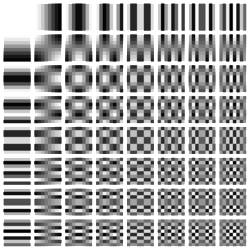
\includegraphics[scale=0.15]{DCT-8x8.png}
\end{center}

\Method[Deblurring an image] A blurred image can be modeled as the 2D-Convolution of the actual image with a small filter. In the 2D-frequency-domain deblurring equals component wise division.

\section{Fast Fourier Transform}
The DFT of a vector of length $pq$ can be divided in $p$ DFT's of vectors of length $q$. The asymptotic runtime for this special 'divide and conquer' is
$$\FFT(n) \in \BigO(n \log n)$$
Special Case $p=2$: 
$$\DFT(\vv) = \DFT(\vv_{even})+s \DFT(\vv_{odd})$$

\sep
\Def[Toeplitz Matrix] $\mathbf{T}=\left(t_{i j}\right)_{i, j=1}^{n} \in \mathbb{K}^{mn}$
is a Toeplitz matrix if it has constant diagonals given by a vector $\vu \in \K^{m+n-1}$. Note that every circulant matrix is also a Toeplitz matrix.\\

\Lemma[Fast Arithmetic for Toeplitz] \\
\textbf{Vector Multiplication in $\BigO((n+m)\log(n+m))$: }
Construct Circulant Matrix $\MC \in \K^{m+n, m+n}$ s.t.
$$\left[\begin{array}{l} \MT\vx \\ \star \end{array}\right] = \MC \left[\begin{array}{l} \vx \\0\end{array}\right]$$
which can be solved in the frequency domain (Convolution Theorem).

\textbf{LSE Solution in $\BigO(n^2)$: }
The Levinson Algorithm.
